\section{Model}

The model has two modes which are shown in Figure \ref{pmodel}. $x(t)$, $y(t)$, and $z(t)$ represent the population of AD cells, the population of AI cells, and the serum androgen concentration, respectively. The growth dynamics of AD and AI cells are governed by their proliferation rate, apoptosis rate and mutation rate from AD to AI phenotype, depending on androgen concentration $z(t)$. The PSA level $v$ (ng ml$^{-1}$) is defined as $v(t)=x(t)+y(t)$. The treatment is suspended or restarted according to the value of $v$ and ${dv}/{dt}$. In mode $2$ (off-treatment), the androgen concentration is maintained at the normal level $z_0$ by homeostasis. In mode $1$ (on-treatment), the androgen is cleared at a rate $1/\tau$. Table \ref{prostate} lists the values of model parameters.

\begin{figure}[htb]
\centering
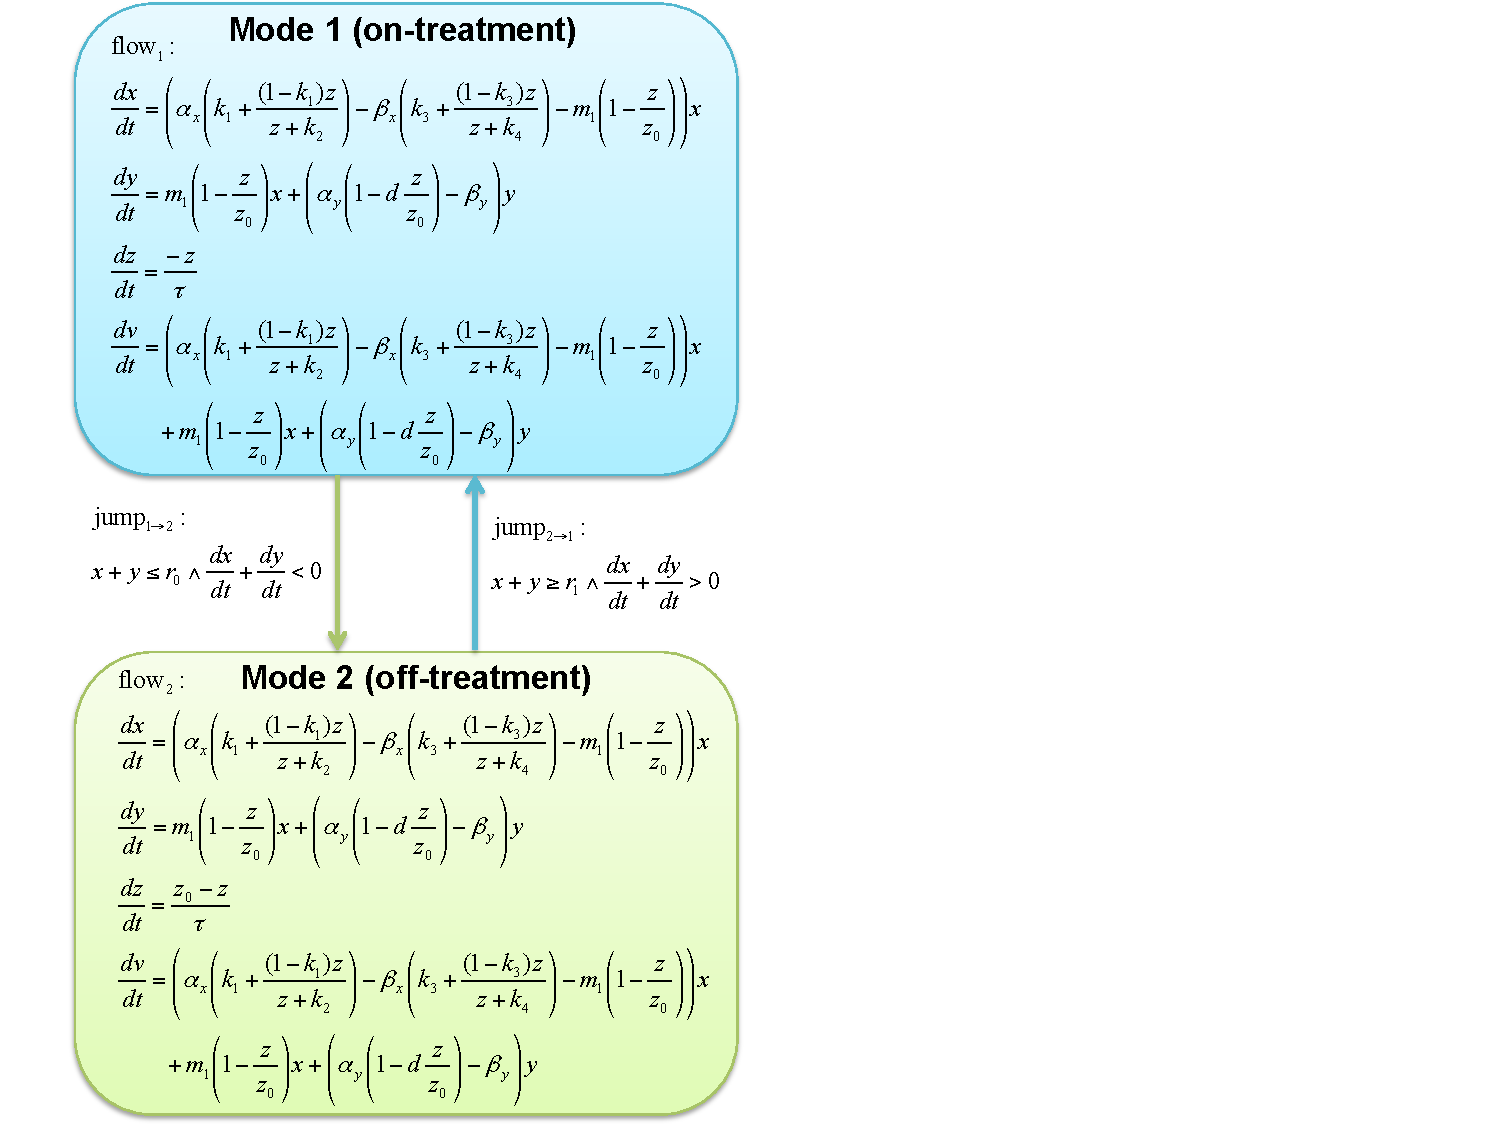
\includegraphics[scale=0.6]{fig-prostate}
\caption{The prostate cancer treatment model.}
\label{pmodel}
 %\vspace{-0.7cm}
\end{figure}

\begin{table}[h]
\caption{Prostate cancer model parameter values\label{prostate}}
\centering
\begin{tabular}{c|c|c}
\hline
Parameter  & Bone metastasis & Lymph node metastasis  \\\hline
$\alpha_x$ & 0.0204 d$^{-1}$ & 0.0168 d$^{-1}$  \\
$\alpha_y$ & 0.0242 d$^{-1}$ & 0.0277 d$^{-1}$  \\
$\beta_x$  & 0.0076 d$^{-1}$ & 0.0085 d$^{-1}$  \\
$\beta_y$  & 0.0168 d$^{-1}$ & 0.0222 d$^{-1}$  \\
$k_1$     & 0.0 nM & 0.0 nM \\
$k_2$     & 2.0 & 2.0  \\
$k_3$     & 8.0 nM & 8.0 nM \\
$k_4$     & 0.5 & 0.5  \\
$m_1$     & 0.00005 d$^{-1}$ & 0.00005 d$^{-1}$  \\
$z_0$     & 20.0 nM & 20.0 nM  \\
$\tau$     & 62.5 d & 62.5 d \\
\hline
\end{tabular}
 %\vspace{-0.7cm}
\end{table}
